%%%%%%%%%%%%  Generated using docx2latex.com  %%%%%%%%%%%%%%

%%%%%%%%%%%%  v2.0.0-beta  %%%%%%%%%%%%%%

\documentclass[12pt]{article}
\usepackage{amsmath}
\usepackage{latexsym}
\usepackage{amsfonts}
\usepackage[normalem]{ulem}
\usepackage{soul}
\usepackage{array}
\usepackage{amssymb}
\usepackage{extarrows}
\usepackage{graphicx}
\usepackage[backend=biber,
style=numeric,
sorting=none,
isbn=false,
doi=false,
url=false,
]{biblatex}\addbibresource{bibliography.bib}

\usepackage{subfig}
\usepackage{wrapfig}
\usepackage{wasysym}
\usepackage{enumitem}
\usepackage{adjustbox}
\usepackage{ragged2e}
\usepackage[svgnames,table]{xcolor}
\usepackage{tikz}
\usepackage{longtable}
\usepackage{changepage}
\usepackage{setspace}
\usepackage{hhline}
\usepackage{multicol}
\usepackage{tabto}
\usepackage{float}
\usepackage{multirow}
\usepackage{makecell}
\usepackage{fancyhdr}
\usepackage[toc,page]{appendix}
\usepackage[hidelinks]{hyperref}
\usetikzlibrary{shapes.symbols,shapes.geometric,shadows,arrows.meta}
\tikzset{>={Latex[width=1.5mm,length=2mm]}}
\usepackage{flowchart}\usepackage[paperheight=11.69in,paperwidth=8.26in,left=1.0in,right=1.0in,top=1.0in,bottom=1.0in,headheight=1in]{geometry}
\usepackage{CJKutf8}
\TabPositions{0.5in,1.0in,1.5in,2.0in,2.5in,3.0in,3.5in,4.0in,4.5in,5.0in,5.5in,6.0in,}

\urlstyle{same}


 %%%%%%%%%%%%  Set Depths for Sections  %%%%%%%%%%%%%%

% 1) Section
% 1.1) SubSection
% 1.1.1) SubSubSection
% 1.1.1.1) Paragraph
% 1.1.1.1.1) Subparagraph


\setcounter{tocdepth}{5}
\setcounter{secnumdepth}{5}


 %%%%%%%%%%%%  Set Depths for Nested Lists created by \begin{enumerate}  %%%%%%%%%%%%%%


\setlistdepth{9}
\renewlist{enumerate}{enumerate}{9}
		\setlist[enumerate,1]{label=\arabic*)}
		\setlist[enumerate,2]{label=\alph*)}
		\setlist[enumerate,3]{label=(\roman*)}
		\setlist[enumerate,4]{label=(\arabic*)}
		\setlist[enumerate,5]{label=(\Alph*)}
		\setlist[enumerate,6]{label=(\Roman*)}
		\setlist[enumerate,7]{label=\arabic*}
		\setlist[enumerate,8]{label=\alph*}
		\setlist[enumerate,9]{label=\roman*}

\renewlist{itemize}{itemize}{9}
		\setlist[itemize]{label=$\cdot$}
		\setlist[itemize,1]{label=\textbullet}
		\setlist[itemize,2]{label=$\circ$}
		\setlist[itemize,3]{label=$\ast$}
		\setlist[itemize,4]{label=$\dagger$}
		\setlist[itemize,5]{label=$\triangleright$}
		\setlist[itemize,6]{label=$\bigstar$}
		\setlist[itemize,7]{label=$\blacklozenge$}
		\setlist[itemize,8]{label=$\prime$}

\setlength{\topsep}{0pt}\setlength{\parindent}{0pt}
\renewcommand{\arraystretch}{1.3}


%%%%%%%%%%%%%%%%%%%% Document code starts here %%%%%%%%%%%%%%%%%%%%



\begin{document}
\begin{CJK*}{UTF8}{gbsn}
\section{环境参数对飞机设计的影响}
\subsection{引言}
商用飞机从设计伊始到退出市场运营,这一过程受到众多环境因素的影响,商用飞机的经济性评估也受到环境因素的影响。在商用飞机的概念设计阶段就对这些环境参数进行考虑能够得到更加全面以及具有前瞻性的飞机设计方案。本章将对飞机的部分环境参数对飞机设计与评估的影响进行探索,搭建了与环境参数耦合的飞机设计程序,并将对环境参数进行相关飞机属性的敏感性分析。\par

\subsection{环境因素与飞机设计程序的耦合}
飞机设计中相关的环境影响因素包括航空公司的运营参数的影响,机场环境参数的影响,航线网络参数的影响,宏观经济环境参数的影响,制造商运营参数的影响以及与设计活动相关参数的影响。这些参数在X节做了介绍。本章将研究将环境参数与飞机设计相耦合的方法以及对相关的环境参数进行敏感性分析。\par



%%%%%%%%%%%%%%%%%%%% Figure/Image No: 1 starts here %%%%%%%%%%%%%%%%%%%%

\begin{figure}[H]
	\begin{Center}
		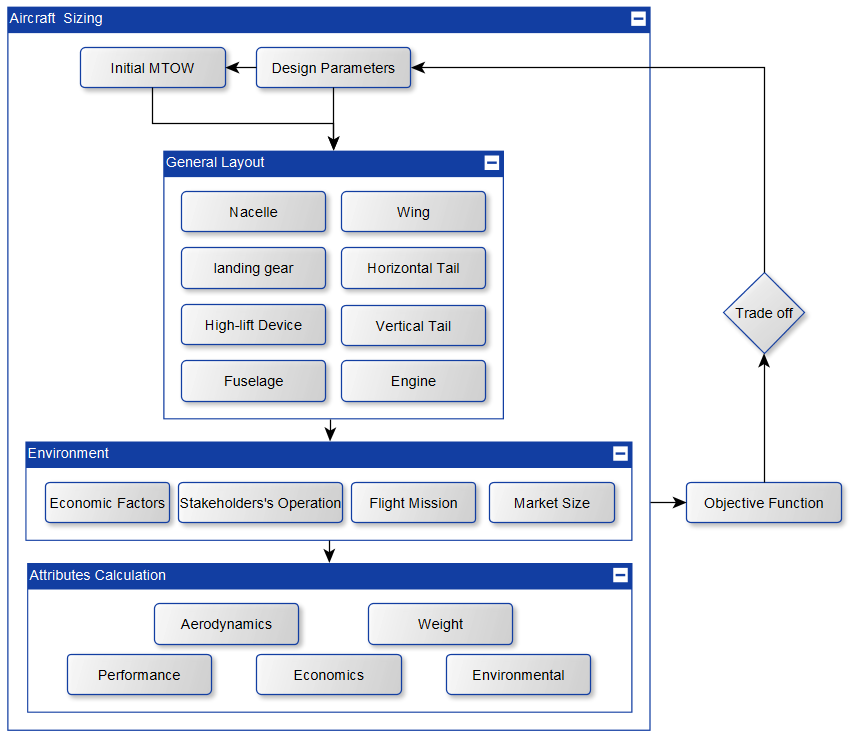
\includegraphics[width=4.06in,height=3.5in]{./media511/image1.png}
	\end{Center}
\end{figure}


%%%%%%%%%%%%%%%%%%%% Figure/Image No: 1 Ends here %%%%%%%%%%%%%%%%%%%%

\par

\begin{Center}
图5-1 与环境参数耦合的飞机设计程序
\end{Center}\par

\begin{Center}
Fig.5-1 Aircraft design program integrated with scenarios
\end{Center}\par


\vspace{\baselineskip}
本研究搭建了与飞机设计环境相互耦合的飞机设计框架,如图5-1所示。在图X中,在对飞机属性的评估之前,包括飞机气动,性能,重量,环保性以及飞机的经济性的估算,首先需要定义并且量化一组环境参数,用这一组环境参数搭建一个完整的环境,进而计算飞机的这些属性。\par

\subsubsection{航空公司运营参数的影响}
航空公司的运营参数,包括飞机的年飞行小时数,座位数与座位布局,机票价格,乘务人员的数量配置等。这些参数会对飞机的经济性评估产生影响,进而对飞机设计方案的权衡与优化产生影响。\par

\begin{enumerate}
	\item \textbf{飞机的年飞行小时数}\par

飞机的年飞行小时数会影响飞机利用率与直接使用成本,进而对飞机的剩余价值产生影响,年飞行小时数对飞机经济性的影响如图5-2所示。\par



%%%%%%%%%%%%%%%%%%%% Figure/Image No: 2 starts here %%%%%%%%%%%%%%%%%%%%

\begin{figure}[H]
	\begin{Center}
		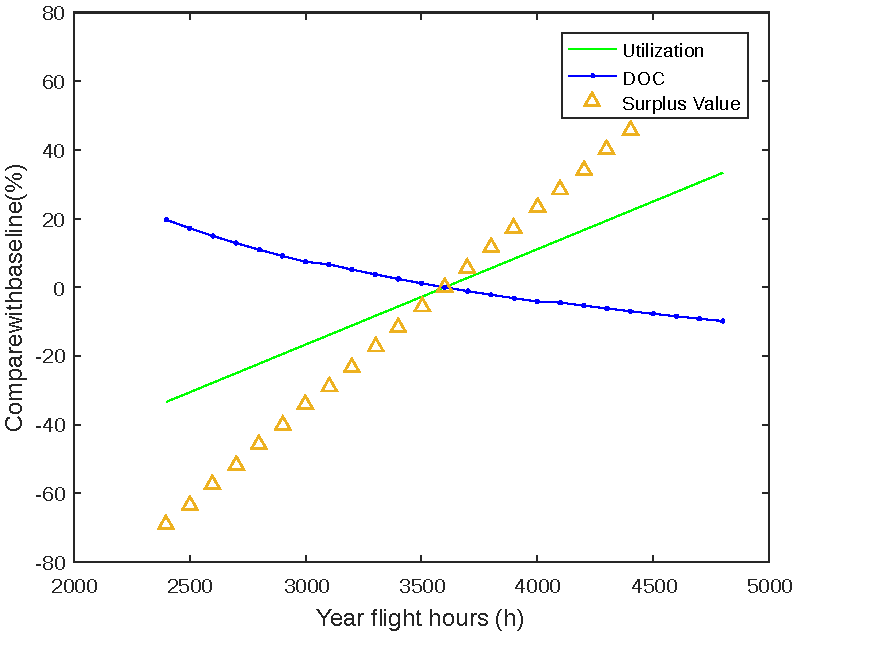
\includegraphics[width=3.62in,height=2.71in]{./media511/image2.pdf}
	\end{Center}
\end{figure}


%%%%%%%%%%%%%%%%%%%% Figure/Image No: 2 Ends here %%%%%%%%%%%%%%%%%%%%

\par

\begin{Center}
图5-2 年飞行小时数对飞机经济性的影响
\end{Center}\par

\begin{Center}
Fig.5-2 Year flight hours sensitivity study 
\end{Center}\par


\vspace{\baselineskip}
在图5-2中,飞机的年飞机小时数的变化对飞机的利用率产生直接的影响,飞机的利用率随着年飞行小时数的增加而增加。飞机每趟飞行的直接使用成本随着年飞行小时数的增加而递减。在剩余价值的计算中,飞机的利用率对剩余价值的计算产生直接的影响,因此剩余价值随着飞机年飞行小时数的增加而增加。\par

	\item \textbf{设计座位数}
\end{enumerate}\par

飞机的座位数会对飞机的制造成本与运营成本产生影响,同时也对飞机的盈利性产生影响。飞机的设计座位数对飞机设计的影响如图5-3所示。\par



%%%%%%%%%%%%%%%%%%%% Figure/Image No: 3 starts here %%%%%%%%%%%%%%%%%%%%

\begin{figure}[H]
	\begin{Center}
		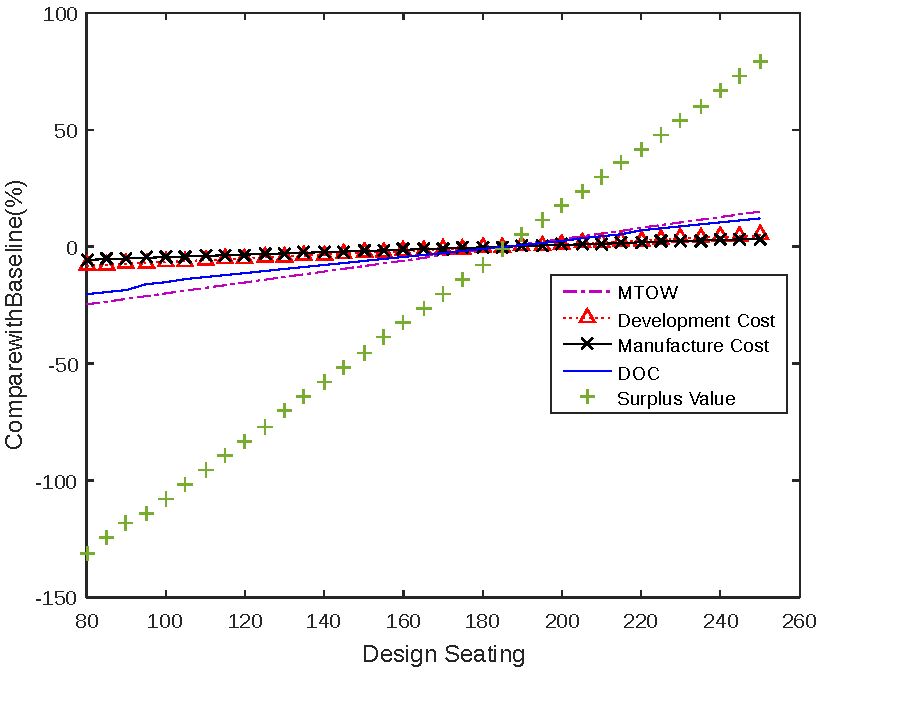
\includegraphics[width=3.33in,height=2.77in]{./media511/image3.pdf}
	\end{Center}
\end{figure}


%%%%%%%%%%%%%%%%%%%% Figure/Image No: 3 Ends here %%%%%%%%%%%%%%%%%%%%

\par

\begin{Center}
图5-3 设计座位数的影响
\end{Center}\par

\begin{Center}
Fig.5-3 Year flight hours sensitivity study 
\end{Center}\par


\vspace{\baselineskip}
从图5-3可以得出,飞机的座位数对飞机的重量产生影响,进而对飞机的研发成本与制造成本产生影响。设计座位数增加,飞机的空机重量与最大起飞重量增加,飞机的研发成本与制造成本上升。飞机的座位数增加,飞机的运行成本上升。当飞机的座位数增加,保持机票价格不变,飞机的剩余价值并没有因为重量,研发成本,制造成本以及使用成本的增加而减少。相反,飞机座位数的增加使得飞机盈利性增加对剩余价值的增益大于重量与成本增加所带来的负面影响,因此飞机的剩余价值提升。\par

\end{CJK*}

\printbibliography
\end{document}